% Options for packages loaded elsewhere
\PassOptionsToPackage{unicode}{hyperref}
\PassOptionsToPackage{hyphens}{url}
%
\documentclass[
  ignorenonframetext,
]{beamer}
\usepackage{pgfpages}
\setbeamertemplate{caption}[numbered]
\setbeamertemplate{caption label separator}{: }
\setbeamercolor{caption name}{fg=normal text.fg}
\beamertemplatenavigationsymbolsempty
% Prevent slide breaks in the middle of a paragraph
\widowpenalties 1 10000
\raggedbottom
\setbeamertemplate{part page}{
  \centering
  \begin{beamercolorbox}[sep=16pt,center]{part title}
    \usebeamerfont{part title}\insertpart\par
  \end{beamercolorbox}
}
\setbeamertemplate{section page}{
  \centering
  \begin{beamercolorbox}[sep=12pt,center]{part title}
    \usebeamerfont{section title}\insertsection\par
  \end{beamercolorbox}
}
\setbeamertemplate{subsection page}{
  \centering
  \begin{beamercolorbox}[sep=8pt,center]{part title}
    \usebeamerfont{subsection title}\insertsubsection\par
  \end{beamercolorbox}
}
\AtBeginPart{
  \frame{\partpage}
}
\AtBeginSection{
  \ifbibliography
  \else
    \frame{\sectionpage}
  \fi
}
\AtBeginSubsection{
  \frame{\subsectionpage}
}
\usepackage{amsmath,amssymb}
\usepackage{iftex}
\ifPDFTeX
  \usepackage[T1]{fontenc}
  \usepackage[utf8]{inputenc}
  \usepackage{textcomp} % provide euro and other symbols
\else % if luatex or xetex
  \usepackage{unicode-math} % this also loads fontspec
  \defaultfontfeatures{Scale=MatchLowercase}
  \defaultfontfeatures[\rmfamily]{Ligatures=TeX,Scale=1}
\fi
\usepackage{lmodern}
\ifPDFTeX\else
  % xetex/luatex font selection
\fi
% Use upquote if available, for straight quotes in verbatim environments
\IfFileExists{upquote.sty}{\usepackage{upquote}}{}
\IfFileExists{microtype.sty}{% use microtype if available
  \usepackage[]{microtype}
  \UseMicrotypeSet[protrusion]{basicmath} % disable protrusion for tt fonts
}{}
\makeatletter
\@ifundefined{KOMAClassName}{% if non-KOMA class
  \IfFileExists{parskip.sty}{%
    \usepackage{parskip}
  }{% else
    \setlength{\parindent}{0pt}
    \setlength{\parskip}{6pt plus 2pt minus 1pt}}
}{% if KOMA class
  \KOMAoptions{parskip=half}}
\makeatother
\usepackage{xcolor}
\newif\ifbibliography
\usepackage{color}
\usepackage{fancyvrb}
\newcommand{\VerbBar}{|}
\newcommand{\VERB}{\Verb[commandchars=\\\{\}]}
\DefineVerbatimEnvironment{Highlighting}{Verbatim}{commandchars=\\\{\}}
% Add ',fontsize=\small' for more characters per line
\usepackage{framed}
\definecolor{shadecolor}{RGB}{248,248,248}
\newenvironment{Shaded}{\begin{snugshade}}{\end{snugshade}}
\newcommand{\AlertTok}[1]{\textcolor[rgb]{0.94,0.16,0.16}{#1}}
\newcommand{\AnnotationTok}[1]{\textcolor[rgb]{0.56,0.35,0.01}{\textbf{\textit{#1}}}}
\newcommand{\AttributeTok}[1]{\textcolor[rgb]{0.13,0.29,0.53}{#1}}
\newcommand{\BaseNTok}[1]{\textcolor[rgb]{0.00,0.00,0.81}{#1}}
\newcommand{\BuiltInTok}[1]{#1}
\newcommand{\CharTok}[1]{\textcolor[rgb]{0.31,0.60,0.02}{#1}}
\newcommand{\CommentTok}[1]{\textcolor[rgb]{0.56,0.35,0.01}{\textit{#1}}}
\newcommand{\CommentVarTok}[1]{\textcolor[rgb]{0.56,0.35,0.01}{\textbf{\textit{#1}}}}
\newcommand{\ConstantTok}[1]{\textcolor[rgb]{0.56,0.35,0.01}{#1}}
\newcommand{\ControlFlowTok}[1]{\textcolor[rgb]{0.13,0.29,0.53}{\textbf{#1}}}
\newcommand{\DataTypeTok}[1]{\textcolor[rgb]{0.13,0.29,0.53}{#1}}
\newcommand{\DecValTok}[1]{\textcolor[rgb]{0.00,0.00,0.81}{#1}}
\newcommand{\DocumentationTok}[1]{\textcolor[rgb]{0.56,0.35,0.01}{\textbf{\textit{#1}}}}
\newcommand{\ErrorTok}[1]{\textcolor[rgb]{0.64,0.00,0.00}{\textbf{#1}}}
\newcommand{\ExtensionTok}[1]{#1}
\newcommand{\FloatTok}[1]{\textcolor[rgb]{0.00,0.00,0.81}{#1}}
\newcommand{\FunctionTok}[1]{\textcolor[rgb]{0.13,0.29,0.53}{\textbf{#1}}}
\newcommand{\ImportTok}[1]{#1}
\newcommand{\InformationTok}[1]{\textcolor[rgb]{0.56,0.35,0.01}{\textbf{\textit{#1}}}}
\newcommand{\KeywordTok}[1]{\textcolor[rgb]{0.13,0.29,0.53}{\textbf{#1}}}
\newcommand{\NormalTok}[1]{#1}
\newcommand{\OperatorTok}[1]{\textcolor[rgb]{0.81,0.36,0.00}{\textbf{#1}}}
\newcommand{\OtherTok}[1]{\textcolor[rgb]{0.56,0.35,0.01}{#1}}
\newcommand{\PreprocessorTok}[1]{\textcolor[rgb]{0.56,0.35,0.01}{\textit{#1}}}
\newcommand{\RegionMarkerTok}[1]{#1}
\newcommand{\SpecialCharTok}[1]{\textcolor[rgb]{0.81,0.36,0.00}{\textbf{#1}}}
\newcommand{\SpecialStringTok}[1]{\textcolor[rgb]{0.31,0.60,0.02}{#1}}
\newcommand{\StringTok}[1]{\textcolor[rgb]{0.31,0.60,0.02}{#1}}
\newcommand{\VariableTok}[1]{\textcolor[rgb]{0.00,0.00,0.00}{#1}}
\newcommand{\VerbatimStringTok}[1]{\textcolor[rgb]{0.31,0.60,0.02}{#1}}
\newcommand{\WarningTok}[1]{\textcolor[rgb]{0.56,0.35,0.01}{\textbf{\textit{#1}}}}
\usepackage{graphicx}
\makeatletter
\def\maxwidth{\ifdim\Gin@nat@width>\linewidth\linewidth\else\Gin@nat@width\fi}
\def\maxheight{\ifdim\Gin@nat@height>\textheight\textheight\else\Gin@nat@height\fi}
\makeatother
% Scale images if necessary, so that they will not overflow the page
% margins by default, and it is still possible to overwrite the defaults
% using explicit options in \includegraphics[width, height, ...]{}
\setkeys{Gin}{width=\maxwidth,height=\maxheight,keepaspectratio}
% Set default figure placement to htbp
\makeatletter
\def\fps@figure{htbp}
\makeatother
\setlength{\emergencystretch}{3em} % prevent overfull lines
\providecommand{\tightlist}{%
  \setlength{\itemsep}{0pt}\setlength{\parskip}{0pt}}
\setcounter{secnumdepth}{-\maxdimen} % remove section numbering
\ifLuaTeX
  \usepackage{selnolig}  % disable illegal ligatures
\fi
\IfFileExists{bookmark.sty}{\usepackage{bookmark}}{\usepackage{hyperref}}
\IfFileExists{xurl.sty}{\usepackage{xurl}}{} % add URL line breaks if available
\urlstyle{same}
\hypersetup{
  pdftitle={Introduction to Infectious Disease Modelling},
  pdfauthor={Roel Bakker},
  hidelinks,
  pdfcreator={LaTeX via pandoc}}

\title{Introduction to Infectious Disease Modelling}
\author{Roel Bakker}
\date{16-April-2024}

\begin{document}
\frame{\titlepage}

\begin{frame}{Agenda}
\protect\hypertarget{agenda}{}
\begin{itemize}
\tightlist
\item
  Round of introduction
\item
  \protect\hyperlink{install-r-and-rstudio}{Install R and RStudio}
\item
  \protect\hyperlink{introduction-to-r}{Introduction to R}
\item
  \href{./R/R_lab.R}{R Lab}
\item
  Q \& A
\item
  Coffee Break
\item
  \protect\hyperlink{sir-model}{SIR Model}
\item
  \protect\hyperlink{sir-model-in-rstudio}{SIR Model in RStudio}
\item
  \protect\hyperlink{background-on-differential-equations}{Background on
  Differential Equations}
\item
  Q \& A
\end{itemize}
\end{frame}

\begin{frame}[fragile]{Install R and RStudio}
\protect\hypertarget{install-r-and-rstudio}{}
\begin{itemize}
\tightlist
\item
  download R from r-project.org
  {[}\url{http://cran.at.r-project.org/}{]}
\item
  download RStudio Desktop from rstudio.org
  {[}\url{http://www.rstudio.com/ide/download/}{]}
\item
  install both R and RStudio
\item
  test successful installation with:
\end{itemize}

\begin{Shaded}
\begin{Highlighting}[]
\FunctionTok{demo}\NormalTok{(graphics)}
\end{Highlighting}
\end{Shaded}
\end{frame}

\begin{frame}[fragile]{Introduction to R}
\protect\hypertarget{introduction-to-r}{}
\begin{Shaded}
\begin{Highlighting}[]
\NormalTok{x }\OtherTok{=} \FunctionTok{rnorm}\NormalTok{(}\DecValTok{12}\NormalTok{, }\AttributeTok{mean =} \SpecialCharTok{{-}}\DecValTok{5}\NormalTok{)}
\NormalTok{x }
\end{Highlighting}
\end{Shaded}

\begin{verbatim}
##  [1] -4.690392 -5.811608 -3.480207 -4.057497 -4.567462 -5.748974 -3.136513
##  [8] -4.358232 -4.912106 -6.604042 -4.932776 -5.783031
\end{verbatim}

\begin{Shaded}
\begin{Highlighting}[]
\FunctionTok{mean}\NormalTok{(x)}
\end{Highlighting}
\end{Shaded}

\begin{verbatim}
## [1] -4.840237
\end{verbatim}

\begin{Shaded}
\begin{Highlighting}[]
\FunctionTok{summary}\NormalTok{(x)}
\end{Highlighting}
\end{Shaded}

\begin{verbatim}
##    Min. 1st Qu.  Median    Mean 3rd Qu.    Max. 
##  -6.604  -5.757  -4.801  -4.840  -4.283  -3.137
\end{verbatim}

\begin{Shaded}
\begin{Highlighting}[]
\CommentTok{\# Draw a histogram}
\FunctionTok{hist}\NormalTok{(x)}
\end{Highlighting}
\end{Shaded}

\includegraphics{Introduction-to-infectious-disease-modelling-session-1_files/figure-beamer/unnamed-chunk-1-1.pdf}

\begin{Shaded}
\begin{Highlighting}[]
\CommentTok{\# with more values}
\FunctionTok{hist}\NormalTok{(}\FunctionTok{rnorm}\NormalTok{(}\DecValTok{1000000}\NormalTok{,}\AttributeTok{mean=}\DecValTok{4}\NormalTok{),}\AttributeTok{breaks=}\DecValTok{100}\NormalTok{,}\AttributeTok{col=}\StringTok{"red"}\NormalTok{)}
\end{Highlighting}
\end{Shaded}

\includegraphics{Introduction-to-infectious-disease-modelling-session-1_files/figure-beamer/unnamed-chunk-1-2.pdf}
\end{frame}

\begin{frame}[fragile]{Working on the R command-line}
\protect\hypertarget{working-on-the-r-command-line}{}
\begin{itemize}
\tightlist
\item
  \^{} v arrow keys to navigate your command history
\item
  \textless- -\textgreater{} arrow keys to edit the command-line
\item
  you can save the command history:
\end{itemize}

\begin{verbatim}
history()
\end{verbatim}

\begin{itemize}
\tightlist
\item
  TAB for object/file completion
\end{itemize}

\begin{verbatim}
df = read.csv("data   ")
\end{verbatim}
\end{frame}

\begin{frame}[fragile]{1.1 Expressions}
\protect\hypertarget{expressions}{}
\begin{Shaded}
\begin{Highlighting}[]
\DecValTok{2}\SpecialCharTok{+}\DecValTok{3}
\end{Highlighting}
\end{Shaded}

\begin{verbatim}
## [1] 5
\end{verbatim}

\begin{Shaded}
\begin{Highlighting}[]
\DecValTok{4}\SpecialCharTok{*}\DecValTok{5}
\end{Highlighting}
\end{Shaded}

\begin{verbatim}
## [1] 20
\end{verbatim}

\begin{Shaded}
\begin{Highlighting}[]
\DecValTok{3}\SpecialCharTok{\^{}}\NormalTok{(}\DecValTok{1}\SpecialCharTok{/}\DecValTok{2}\NormalTok{)}
\end{Highlighting}
\end{Shaded}

\begin{verbatim}
## [1] 1.732051
\end{verbatim}

\begin{Shaded}
\begin{Highlighting}[]
\DecValTok{2}\SpecialCharTok{\^{}}\DecValTok{8}
\end{Highlighting}
\end{Shaded}

\begin{verbatim}
## [1] 256
\end{verbatim}

R \textbf{evaluates} these expressions, i.e.~determines the
\textbf{value} of these expressions
\end{frame}

\begin{frame}[fragile]{1.2 Expressions evaluating to logical values}
\protect\hypertarget{expressions-evaluating-to-logical-values}{}
\begin{Shaded}
\begin{Highlighting}[]
\DecValTok{2} \SpecialCharTok{\textless{}} \DecValTok{3}   
\end{Highlighting}
\end{Shaded}

\begin{verbatim}
## [1] TRUE
\end{verbatim}

\begin{Shaded}
\begin{Highlighting}[]
\DecValTok{1} \SpecialCharTok{\textgreater{}} \DecValTok{10}  
\end{Highlighting}
\end{Shaded}

\begin{verbatim}
## [1] FALSE
\end{verbatim}

\begin{Shaded}
\begin{Highlighting}[]
\DecValTok{5} \SpecialCharTok{==} \DecValTok{5}   
\end{Highlighting}
\end{Shaded}

\begin{verbatim}
## [1] TRUE
\end{verbatim}

\begin{Shaded}
\begin{Highlighting}[]
\DecValTok{5} \SpecialCharTok{!=} \DecValTok{5}
\end{Highlighting}
\end{Shaded}

\begin{verbatim}
## [1] FALSE
\end{verbatim}
\end{frame}

\begin{frame}[fragile]
Short for \textbf{TRUE} and \textbf{FALSE}

\begin{Shaded}
\begin{Highlighting}[]
\NormalTok{T}
\end{Highlighting}
\end{Shaded}

\begin{verbatim}
## [1] TRUE
\end{verbatim}

\begin{Shaded}
\begin{Highlighting}[]
\NormalTok{F}
\end{Highlighting}
\end{Shaded}

\begin{verbatim}
## [1] FALSE
\end{verbatim}
\end{frame}

\begin{frame}{1.3 Variables}
\protect\hypertarget{variables}{}
Every variable has a \textbf{name} and a \textbf{type}.

R has the following data types: \textbf{character}, \textbf{numeric},
\textbf{integer} and \textbf{logical}.

The name of a variable may contain

\begin{itemize}
\tightlist
\item
  letters (upper/lower case matters)
\item
  digits
\item
  periods
\item
  underscores and
\item
  should start with a letter
\end{itemize}
\end{frame}

\begin{frame}[fragile]
Variables do not need to be declared first.

A variable is assigned a value in an `assignment' statement (in addition
to \textbf{=} it is possible to use \textbf{\textless-} as assignment
operator)

\begin{Shaded}
\begin{Highlighting}[]
\NormalTok{x }\OtherTok{=} \DecValTok{200}
\NormalTok{half.x  }\OtherTok{=}\NormalTok{  x}\SpecialCharTok{/}\DecValTok{2}
\NormalTok{half.x}
\end{Highlighting}
\end{Shaded}

\begin{verbatim}
## [1] 100
\end{verbatim}

\begin{Shaded}
\begin{Highlighting}[]
\NormalTok{y }\OtherTok{\textless{}{-}} \FloatTok{12.3}
\NormalTok{y }
\end{Highlighting}
\end{Shaded}

\begin{verbatim}
## [1] 12.3
\end{verbatim}
\end{frame}

\begin{frame}[fragile]{1.3.1 character}
\protect\hypertarget{character}{}
The class() function is used to lookup the type of a variable.

\begin{Shaded}
\begin{Highlighting}[]
\NormalTok{firstName }\OtherTok{=} \StringTok{"John"}
\FunctionTok{class}\NormalTok{(firstName)}
\end{Highlighting}
\end{Shaded}

\begin{verbatim}
## [1] "character"
\end{verbatim}

\begin{Shaded}
\begin{Highlighting}[]
\NormalTok{firstName}
\end{Highlighting}
\end{Shaded}

\begin{verbatim}
## [1] "John"
\end{verbatim}
\end{frame}

\begin{frame}[fragile]{1.3.2 numeric}
\protect\hypertarget{numeric}{}
\begin{Shaded}
\begin{Highlighting}[]
\NormalTok{heightInCm }\OtherTok{=} \FloatTok{178.2}
\FunctionTok{class}\NormalTok{(heightInCm)}
\end{Highlighting}
\end{Shaded}

\begin{verbatim}
## [1] "numeric"
\end{verbatim}

\begin{Shaded}
\begin{Highlighting}[]
\NormalTok{heightInCm}
\end{Highlighting}
\end{Shaded}

\begin{verbatim}
## [1] 178.2
\end{verbatim}
\end{frame}

\begin{frame}[fragile]{1.3.3 integer}
\protect\hypertarget{integer}{}
\begin{Shaded}
\begin{Highlighting}[]
\NormalTok{numberOfChildren }\OtherTok{=} \DecValTok{2}
\FunctionTok{class}\NormalTok{(numberOfChildren)}
\end{Highlighting}
\end{Shaded}

\begin{verbatim}
## [1] "numeric"
\end{verbatim}

\begin{Shaded}
\begin{Highlighting}[]
\NormalTok{numberOfChildren }\OtherTok{=}\NormalTok{ 2L }\CommentTok{\# number of children should be integer}
\FunctionTok{class}\NormalTok{(numberOfChildren)}
\end{Highlighting}
\end{Shaded}

\begin{verbatim}
## [1] "integer"
\end{verbatim}

\begin{Shaded}
\begin{Highlighting}[]
\NormalTok{numberOfChildren}
\end{Highlighting}
\end{Shaded}

\begin{verbatim}
## [1] 2
\end{verbatim}
\end{frame}

\begin{frame}[fragile]{1.3.4 logical}
\protect\hypertarget{logical}{}
\begin{Shaded}
\begin{Highlighting}[]
\NormalTok{RisFun }\OtherTok{=}\NormalTok{ T}
\FunctionTok{class}\NormalTok{(RisFun)}
\end{Highlighting}
\end{Shaded}

\begin{verbatim}
## [1] "logical"
\end{verbatim}

\begin{Shaded}
\begin{Highlighting}[]
\NormalTok{RisFun}
\end{Highlighting}
\end{Shaded}

\begin{verbatim}
## [1] TRUE
\end{verbatim}
\end{frame}

\begin{frame}[fragile]{1.3.5 Casting (coercion)}
\protect\hypertarget{casting-coercion}{}
``as'' can be used to cast to a different type:

\begin{Shaded}
\begin{Highlighting}[]
\NormalTok{y }\OtherTok{=} \FunctionTok{as.integer}\NormalTok{(}\FloatTok{3.9}\NormalTok{)}
\FunctionTok{class}\NormalTok{(y)}
\end{Highlighting}
\end{Shaded}

\begin{verbatim}
## [1] "integer"
\end{verbatim}

\begin{Shaded}
\begin{Highlighting}[]
\NormalTok{y }\CommentTok{\# the value of y is truncated}
\end{Highlighting}
\end{Shaded}

\begin{verbatim}
## [1] 3
\end{verbatim}

\begin{Shaded}
\begin{Highlighting}[]
\NormalTok{x }\OtherTok{=} \FunctionTok{as.character}\NormalTok{(}\DecValTok{33}\NormalTok{)}
\FunctionTok{class}\NormalTok{(x)}
\end{Highlighting}
\end{Shaded}

\begin{verbatim}
## [1] "character"
\end{verbatim}

\begin{Shaded}
\begin{Highlighting}[]
\NormalTok{x}
\end{Highlighting}
\end{Shaded}

\begin{verbatim}
## [1] "33"
\end{verbatim}
\end{frame}

\begin{frame}[fragile]{1.4 Functions}
\protect\hypertarget{functions}{}
A function can be called with the name of the function followed by the
arguments of the function:

\begin{Shaded}
\begin{Highlighting}[]
\FunctionTok{max}\NormalTok{(}\DecValTok{9}\NormalTok{,}\DecValTok{3}\NormalTok{,}\DecValTok{4}\NormalTok{,}\DecValTok{2}\NormalTok{,}\DecValTok{11}\NormalTok{,}\DecValTok{2}\NormalTok{)}
\end{Highlighting}
\end{Shaded}

\begin{verbatim}
## [1] 11
\end{verbatim}

\begin{Shaded}
\begin{Highlighting}[]
\FunctionTok{sum}\NormalTok{(}\DecValTok{2}\NormalTok{,}\DecValTok{3}\NormalTok{,}\DecValTok{4}\NormalTok{)}
\end{Highlighting}
\end{Shaded}

\begin{verbatim}
## [1] 9
\end{verbatim}

\begin{Shaded}
\begin{Highlighting}[]
\FunctionTok{prod}\NormalTok{(}\DecValTok{5}\NormalTok{,}\DecValTok{6}\NormalTok{,}\DecValTok{7}\NormalTok{)}
\end{Highlighting}
\end{Shaded}

\begin{verbatim}
## [1] 210
\end{verbatim}
\end{frame}

\begin{frame}[fragile]{1.5 Help}
\protect\hypertarget{help}{}
\begin{verbatim}
? sum
?? product
\end{verbatim}
\end{frame}

\begin{frame}[fragile]{1.6 Files}
\protect\hypertarget{files}{}
\begin{itemize}
\tightlist
\item
  dir() shows the files in the working directory
\item
  ls() shows the variables defined
\end{itemize}

\begin{verbatim}
dir()
ls()
\end{verbatim}
\end{frame}

\begin{frame}[fragile]{2.1 Vectors: what is a vector?}
\protect\hypertarget{vectors-what-is-a-vector}{}
A vector is an ordered collection of values of the same type

\begin{Shaded}
\begin{Highlighting}[]
\NormalTok{lengths }\OtherTok{=} \FunctionTok{c}\NormalTok{ (}\FloatTok{178.2}\NormalTok{, }\FloatTok{180.2}\NormalTok{, }\FloatTok{177.4}\NormalTok{) }\DocumentationTok{\#\# c for "combine"}
\NormalTok{lengths}
\end{Highlighting}
\end{Shaded}

\begin{verbatim}
## [1] 178.2 180.2 177.4
\end{verbatim}

\begin{Shaded}
\begin{Highlighting}[]
\NormalTok{firstNames }\OtherTok{=} \FunctionTok{c}\NormalTok{ (}\StringTok{"John"}\NormalTok{,}\StringTok{"Peter"}\NormalTok{,}\StringTok{"James"}\NormalTok{,}\StringTok{"Mary"}\NormalTok{)}
\NormalTok{firstNames}
\end{Highlighting}
\end{Shaded}

\begin{verbatim}
## [1] "John"  "Peter" "James" "Mary"
\end{verbatim}

Vector of length 1

R works with vectors by default.\\
A variable with one value is a vector of length 1.

\begin{Shaded}
\begin{Highlighting}[]
\NormalTok{x }\OtherTok{=} \FunctionTok{c}\NormalTok{(}\DecValTok{10}\NormalTok{,}\DecValTok{20}\NormalTok{,}\DecValTok{30}\NormalTok{)}
\NormalTok{x}
\end{Highlighting}
\end{Shaded}

\begin{verbatim}
## [1] 10 20 30
\end{verbatim}

\begin{Shaded}
\begin{Highlighting}[]
\FunctionTok{length}\NormalTok{(x) }
\end{Highlighting}
\end{Shaded}

\begin{verbatim}
## [1] 3
\end{verbatim}

\begin{Shaded}
\begin{Highlighting}[]
\NormalTok{y }\OtherTok{=} \DecValTok{33}
\FunctionTok{length}\NormalTok{(y)}
\end{Highlighting}
\end{Shaded}

\begin{verbatim}
## [1] 1
\end{verbatim}

\begin{Shaded}
\begin{Highlighting}[]
\NormalTok{y[}\DecValTok{1}\NormalTok{]}
\end{Highlighting}
\end{Shaded}

\begin{verbatim}
## [1] 33
\end{verbatim}
\end{frame}

\begin{frame}[fragile]{2.2 Sequence vectors}
\protect\hypertarget{sequence-vectors}{}
\begin{Shaded}
\begin{Highlighting}[]
\NormalTok{z }\OtherTok{=} \DecValTok{1}\SpecialCharTok{:}\DecValTok{10}
\NormalTok{z}
\end{Highlighting}
\end{Shaded}

\begin{verbatim}
##  [1]  1  2  3  4  5  6  7  8  9 10
\end{verbatim}

\begin{Shaded}
\begin{Highlighting}[]
\NormalTok{z }\OtherTok{=} \FunctionTok{seq}\NormalTok{(}\DecValTok{1}\NormalTok{,}\DecValTok{5}\NormalTok{)}
\NormalTok{z }\OtherTok{=} \FunctionTok{seq}\NormalTok{(}\AttributeTok{from=}\DecValTok{1}\NormalTok{,}\AttributeTok{to=}\DecValTok{5}\NormalTok{,}\AttributeTok{by=}\DecValTok{1}\SpecialCharTok{/}\DecValTok{3}\NormalTok{)}
\NormalTok{z}
\end{Highlighting}
\end{Shaded}

\begin{verbatim}
##  [1] 1.000000 1.333333 1.666667 2.000000 2.333333 2.666667 3.000000 3.333333
##  [9] 3.666667 4.000000 4.333333 4.666667 5.000000
\end{verbatim}

\begin{Shaded}
\begin{Highlighting}[]
\DecValTok{9}\SpecialCharTok{:}\DecValTok{5}
\end{Highlighting}
\end{Shaded}

\begin{verbatim}
## [1] 9 8 7 6 5
\end{verbatim}
\end{frame}

\begin{frame}[fragile]{2.3 Vectors: selecting elements}
\protect\hypertarget{vectors-selecting-elements}{}
\begin{Shaded}
\begin{Highlighting}[]
\NormalTok{x }\OtherTok{=} \DecValTok{100}\SpecialCharTok{:}\DecValTok{120}
\NormalTok{x[}\DecValTok{1}\NormalTok{]           }\DocumentationTok{\#\# the first element is element nr 1 (not 0 as in C or Python!!) }
\end{Highlighting}
\end{Shaded}

\begin{verbatim}
## [1] 100
\end{verbatim}

\begin{Shaded}
\begin{Highlighting}[]
\NormalTok{x[}\FunctionTok{c}\NormalTok{(}\DecValTok{12}\NormalTok{,}\DecValTok{14}\NormalTok{)]    }\DocumentationTok{\#\# elements 12 and 14}
\end{Highlighting}
\end{Shaded}

\begin{verbatim}
## [1] 111 113
\end{verbatim}

\begin{Shaded}
\begin{Highlighting}[]
\NormalTok{x[}\DecValTok{1}\SpecialCharTok{:}\DecValTok{5}\NormalTok{]         }\DocumentationTok{\#\# elements 1 thru 5}
\end{Highlighting}
\end{Shaded}

\begin{verbatim}
## [1] 100 101 102 103 104
\end{verbatim}

\begin{Shaded}
\begin{Highlighting}[]
\NormalTok{x[}\SpecialCharTok{{-}}\FunctionTok{c}\NormalTok{(}\DecValTok{1}\NormalTok{,}\DecValTok{3}\NormalTok{,}\DecValTok{5}\NormalTok{,}\DecValTok{7}\NormalTok{)] }\DocumentationTok{\#\# excludes elements 1, 3, 5 and 7 }
\end{Highlighting}
\end{Shaded}

\begin{verbatim}
##  [1] 101 103 105 107 108 109 110 111 112 113 114 115 116 117 118 119 120
\end{verbatim}
\end{frame}

\begin{frame}[fragile]{2.4 Vectors: assigning values to elements}
\protect\hypertarget{vectors-assigning-values-to-elements}{}
\begin{Shaded}
\begin{Highlighting}[]
\NormalTok{x }\OtherTok{=} \FunctionTok{rep}\NormalTok{(}\DecValTok{0}\NormalTok{,}\DecValTok{10}\NormalTok{)}
\NormalTok{x [}\DecValTok{1}\SpecialCharTok{:} \DecValTok{3}\NormalTok{] }\OtherTok{=} \DecValTok{2}
\NormalTok{x [}\DecValTok{5}\SpecialCharTok{:} \DecValTok{6}\NormalTok{] }\OtherTok{=} \FunctionTok{c}\NormalTok{(}\DecValTok{5}\NormalTok{,}\ConstantTok{NA}\NormalTok{)}
\NormalTok{x [}\DecValTok{7}\SpecialCharTok{:}\DecValTok{10}\NormalTok{] }\OtherTok{=} \FunctionTok{c}\NormalTok{(}\DecValTok{1}\NormalTok{,}\DecValTok{9}\NormalTok{)}
\NormalTok{x}
\end{Highlighting}
\end{Shaded}

\begin{verbatim}
##  [1]  2  2  2  0  5 NA  1  9  1  9
\end{verbatim}
\end{frame}

\begin{frame}[fragile]{2.5 Vectors: indexing elements by name}
\protect\hypertarget{vectors-indexing-elements-by-name}{}
\begin{Shaded}
\begin{Highlighting}[]
\NormalTok{cc }\OtherTok{=} \FunctionTok{c}\NormalTok{(}\DecValTok{1200}\NormalTok{,}\DecValTok{1800}\NormalTok{,}\DecValTok{3500}\NormalTok{)}
\FunctionTok{names}\NormalTok{(cc)}\OtherTok{=}\FunctionTok{c}\NormalTok{(}\StringTok{"VW Polo"}\NormalTok{,}\StringTok{"MG B"}\NormalTok{,}\StringTok{"Rover V8"}\NormalTok{)}
\NormalTok{cc[}\StringTok{"MG B"}\NormalTok{]}
\end{Highlighting}
\end{Shaded}

\begin{verbatim}
## MG B 
## 1800
\end{verbatim}
\end{frame}

\begin{frame}[fragile]{2.6 Vectors: plotting element values}
\protect\hypertarget{vectors-plotting-element-values}{}
\begin{Shaded}
\begin{Highlighting}[]
\NormalTok{cc }\OtherTok{=} \FunctionTok{c}\NormalTok{(}\DecValTok{1200}\NormalTok{,}\DecValTok{1800}\NormalTok{,}\DecValTok{3500}\NormalTok{)}
\FunctionTok{names}\NormalTok{(cc)}\OtherTok{=}\FunctionTok{c}\NormalTok{(}\StringTok{"VW Polo"}\NormalTok{,}\StringTok{"MG B"}\NormalTok{,}\StringTok{"Rover V8"}\NormalTok{)}
\FunctionTok{barplot}\NormalTok{(cc)}
\end{Highlighting}
\end{Shaded}

\includegraphics{Introduction-to-infectious-disease-modelling-session-1_files/figure-beamer/unnamed-chunk-18-1.pdf}
\end{frame}

\begin{frame}[fragile]{2.7 Computation with vectors}
\protect\hypertarget{computation-with-vectors}{}
\begin{Shaded}
\begin{Highlighting}[]
\NormalTok{a }\OtherTok{=} \FunctionTok{c}\NormalTok{(}\DecValTok{1}\NormalTok{,}\DecValTok{2}\NormalTok{,}\DecValTok{3}\NormalTok{) ; a }\OtherTok{=}\NormalTok{ a }\SpecialCharTok{+} \DecValTok{1}
\NormalTok{a}
\end{Highlighting}
\end{Shaded}

\begin{verbatim}
## [1] 2 3 4
\end{verbatim}

\begin{Shaded}
\begin{Highlighting}[]
\NormalTok{a }\OtherTok{=} \DecValTok{1}\SpecialCharTok{:}\DecValTok{3}\NormalTok{ ; b }\OtherTok{=} \DecValTok{4}\SpecialCharTok{:}\DecValTok{2}\NormalTok{ ; c }\OtherTok{=}\NormalTok{ a }\SpecialCharTok{+}\NormalTok{ b}
\NormalTok{c}
\end{Highlighting}
\end{Shaded}

\begin{verbatim}
## [1] 5 5 5
\end{verbatim}

\begin{Shaded}
\begin{Highlighting}[]
\NormalTok{c}\SpecialCharTok{/}\DecValTok{5}
\end{Highlighting}
\end{Shaded}

\begin{verbatim}
## [1] 1 1 1
\end{verbatim}
\end{frame}

\begin{frame}[fragile]{2.8 Comparing vectors}
\protect\hypertarget{comparing-vectors}{}
\begin{Shaded}
\begin{Highlighting}[]
\NormalTok{a }\OtherTok{=} \FunctionTok{c}\NormalTok{(}\DecValTok{1}\NormalTok{,}\DecValTok{2}\NormalTok{,}\DecValTok{3}\NormalTok{)}
\NormalTok{b }\OtherTok{=} \FunctionTok{c}\NormalTok{(}\DecValTok{4}\NormalTok{,}\DecValTok{2}\NormalTok{,}\DecValTok{5}\NormalTok{)}
\NormalTok{a }\SpecialCharTok{==}\NormalTok{ b}
\end{Highlighting}
\end{Shaded}

\begin{verbatim}
## [1] FALSE  TRUE FALSE
\end{verbatim}

The result is a vector of T/F values i.e.~a logical vector ***** \#\#\#
2.9 Logical vectors

If a vector is compared to a single value all elements of that vector
are compared; the result is a logical vector:

\begin{Shaded}
\begin{Highlighting}[]
\NormalTok{x }\OtherTok{=} \DecValTok{1}\SpecialCharTok{:}\DecValTok{5}
\NormalTok{x}\SpecialCharTok{\textgreater{}}\DecValTok{2}
\end{Highlighting}
\end{Shaded}

\begin{verbatim}
## [1] FALSE FALSE  TRUE  TRUE  TRUE
\end{verbatim}
\end{frame}

\begin{frame}[fragile]
A logical vector can be used to select elements of the original vector:

\begin{Shaded}
\begin{Highlighting}[]
\NormalTok{x }\OtherTok{=} \DecValTok{1}\SpecialCharTok{:}\DecValTok{5}
\NormalTok{select }\OtherTok{=}\NormalTok{ x}\SpecialCharTok{\textgreater{}}\DecValTok{2}
\NormalTok{x[select]}
\end{Highlighting}
\end{Shaded}

\begin{verbatim}
## [1] 3 4 5
\end{verbatim}

in SQL: SELECT * FROM NUMBERS WHERE x\textgreater2; ***** \#\#\# 2.9
Logical vectors: more examples

\begin{Shaded}
\begin{Highlighting}[]
\NormalTok{x }\OtherTok{=} \DecValTok{1}\SpecialCharTok{:}\DecValTok{10}
\NormalTok{gt5 }\OtherTok{=}\NormalTok{ (x }\SpecialCharTok{\textgreater{}} \DecValTok{5}\NormalTok{)}
\NormalTok{lt8 }\OtherTok{=}\NormalTok{ (x }\SpecialCharTok{\textless{}} \DecValTok{8}\NormalTok{)}
\NormalTok{x[gt5 }\SpecialCharTok{\&}\NormalTok{ lt8]}
\end{Highlighting}
\end{Shaded}

\begin{verbatim}
## [1] 6 7
\end{verbatim}

Use \& (not \&\&) as `short-circuit' boolean operators may have
unexpected effects in R !! *****

\begin{Shaded}
\begin{Highlighting}[]
\NormalTok{lt5 }\OtherTok{=}\NormalTok{ (x }\SpecialCharTok{\textless{}} \DecValTok{5}\NormalTok{)}
\NormalTok{gt8 }\OtherTok{=}\NormalTok{ (x }\SpecialCharTok{\textgreater{}} \DecValTok{8}\NormalTok{)}
\NormalTok{x[lt5 }\SpecialCharTok{|}\NormalTok{ gt8]}
\end{Highlighting}
\end{Shaded}

\begin{verbatim}
## [1]  1  2  3  4  9 10
\end{verbatim}

Use \textbar{} (not \textbar\textbar)
\end{frame}

\begin{frame}[fragile]{2.10 Applying functions to vectors}
\protect\hypertarget{applying-functions-to-vectors}{}
\begin{Shaded}
\begin{Highlighting}[]
\NormalTok{z }\OtherTok{=} \FunctionTok{c}\NormalTok{(}\DecValTok{9}\NormalTok{,}\DecValTok{49}\NormalTok{,}\DecValTok{16}\NormalTok{,}\DecValTok{36}\NormalTok{)}
\FunctionTok{min}\NormalTok{(z)}
\end{Highlighting}
\end{Shaded}

\begin{verbatim}
## [1] 9
\end{verbatim}

\begin{Shaded}
\begin{Highlighting}[]
\FunctionTok{range}\NormalTok{(z)}
\end{Highlighting}
\end{Shaded}

\begin{verbatim}
## [1]  9 49
\end{verbatim}

\begin{Shaded}
\begin{Highlighting}[]
\FunctionTok{sqrt}\NormalTok{(z)}
\end{Highlighting}
\end{Shaded}

\begin{verbatim}
## [1] 3 7 4 6
\end{verbatim}

\begin{Shaded}
\begin{Highlighting}[]
\FunctionTok{sum}\NormalTok{(z)}
\end{Highlighting}
\end{Shaded}

\begin{verbatim}
## [1] 110
\end{verbatim}

\begin{Shaded}
\begin{Highlighting}[]
\FunctionTok{summary}\NormalTok{(z)}
\end{Highlighting}
\end{Shaded}

\begin{verbatim}
##    Min. 1st Qu.  Median    Mean 3rd Qu.    Max. 
##    9.00   14.25   26.00   27.50   39.25   49.00
\end{verbatim}
\end{frame}

\begin{frame}[fragile]{2.11 Often used functions with vectors}
\protect\hypertarget{often-used-functions-with-vectors}{}
\begin{verbatim}
length()
rev()
sum(), cumsum(), prod(), cumprod()
mean(), sd(), var(), median()
min(), max(), range(), summary()
exp(), log(), sin(), cos(), tan()
round(), ceil(), 
floor(), signif()
sort(), order(), rank()
which(), which.max()
any(), all()
\end{verbatim}
\end{frame}

\begin{frame}[fragile]{2.12 Scatter plots}
\protect\hypertarget{scatter-plots}{}
\begin{Shaded}
\begin{Highlighting}[]
\NormalTok{x }\OtherTok{=} \SpecialCharTok{{-}}\DecValTok{5}\SpecialCharTok{:}\DecValTok{5}
\NormalTok{y }\OtherTok{=}\NormalTok{ x}\SpecialCharTok{\^{}}\DecValTok{2}
\FunctionTok{plot}\NormalTok{(x,y)}
\end{Highlighting}
\end{Shaded}

\includegraphics{Introduction-to-infectious-disease-modelling-session-1_files/figure-beamer/unnamed-chunk-26-1.pdf}
\end{frame}

\begin{frame}[fragile]{2.13 NA (Not Available)}
\protect\hypertarget{na-not-available}{}
NA indicates that a value is not available (cf NULL in SQL)

\begin{Shaded}
\begin{Highlighting}[]
\FunctionTok{barplot}\NormalTok{(}\FunctionTok{c}\NormalTok{(}\DecValTok{25}\NormalTok{,}\ConstantTok{NA}\NormalTok{,}\DecValTok{20}\NormalTok{))}
\end{Highlighting}
\end{Shaded}

\includegraphics{Introduction-to-infectious-disease-modelling-session-1_files/figure-beamer/unnamed-chunk-27-1.pdf}
\end{frame}

\begin{frame}[fragile]
`Missing values' are denoted with NA NA cannot be compared with other
values

\begin{Shaded}
\begin{Highlighting}[]
\FunctionTok{c}\NormalTok{(}\DecValTok{25}\NormalTok{,}\ConstantTok{NA}\NormalTok{,}\DecValTok{20}\NormalTok{) }\SpecialCharTok{==} \FunctionTok{c}\NormalTok{(}\DecValTok{25}\NormalTok{,}\DecValTok{25}\NormalTok{,}\DecValTok{25}\NormalTok{)}
\end{Highlighting}
\end{Shaded}

\begin{verbatim}
## [1]  TRUE    NA FALSE
\end{verbatim}

\begin{Shaded}
\begin{Highlighting}[]
\CommentTok{\# NA == NA \# neither with itself...}
\FunctionTok{is.na}\NormalTok{(}\ConstantTok{NA}\NormalTok{) }\CommentTok{\# the function is.na() is used to test if a value equals NA}
\end{Highlighting}
\end{Shaded}

\begin{verbatim}
## [1] TRUE
\end{verbatim}
\end{frame}

\begin{frame}[fragile]{3.1 Matrices}
\protect\hypertarget{matrices}{}
Matrices have 2 dimensions

\begin{Shaded}
\begin{Highlighting}[]
\NormalTok{m1 }\OtherTok{=} \FunctionTok{matrix}\NormalTok{(}\DecValTok{9}\NormalTok{,}\AttributeTok{nrow=}\DecValTok{3}\NormalTok{,}\AttributeTok{ncol=}\DecValTok{3}\NormalTok{)}
\NormalTok{m2 }\OtherTok{=} \FunctionTok{matrix}\NormalTok{(}\FunctionTok{c}\NormalTok{(}\DecValTok{11}\SpecialCharTok{:}\DecValTok{14}\NormalTok{,}\DecValTok{21}\SpecialCharTok{:}\DecValTok{24}\NormalTok{),}\AttributeTok{nrow=}\DecValTok{2}\NormalTok{,}\AttributeTok{ncol=}\DecValTok{4}\NormalTok{,}\AttributeTok{byrow=}\NormalTok{T)}
\NormalTok{m2}
\end{Highlighting}
\end{Shaded}

\begin{verbatim}
##      [,1] [,2] [,3] [,4]
## [1,]   11   12   13   14
## [2,]   21   22   23   24
\end{verbatim}
\end{frame}

\begin{frame}[fragile]{3.2 Selecting elements of a matrix}
\protect\hypertarget{selecting-elements-of-a-matrix}{}
\begin{Shaded}
\begin{Highlighting}[]
\CommentTok{\# a single element}
\NormalTok{m2[}\DecValTok{1}\NormalTok{,}\DecValTok{3}\NormalTok{]}
\end{Highlighting}
\end{Shaded}

\begin{verbatim}
## [1] 13
\end{verbatim}

\begin{Shaded}
\begin{Highlighting}[]
\CommentTok{\# selecting a column }
\NormalTok{m2[,}\DecValTok{1}\NormalTok{]}
\end{Highlighting}
\end{Shaded}

\begin{verbatim}
## [1] 11 21
\end{verbatim}

\begin{Shaded}
\begin{Highlighting}[]
\CommentTok{\# selecting a row}
\NormalTok{m2[}\DecValTok{2}\NormalTok{,]}
\end{Highlighting}
\end{Shaded}

\begin{verbatim}
## [1] 21 22 23 24
\end{verbatim}
\end{frame}

\begin{frame}[fragile]{3.3 Plotting matrix values}
\protect\hypertarget{plotting-matrix-values}{}
\begin{Shaded}
\begin{Highlighting}[]
\NormalTok{height}\OtherTok{=}\FunctionTok{matrix}\NormalTok{(}\DecValTok{1}\NormalTok{,}\DecValTok{10}\NormalTok{,}\DecValTok{10}\NormalTok{)}
\NormalTok{height[}\DecValTok{4}\SpecialCharTok{:}\DecValTok{6}\NormalTok{,}\DecValTok{4}\SpecialCharTok{:}\DecValTok{6}\NormalTok{]}\OtherTok{=}\DecValTok{5}
\NormalTok{height}
\end{Highlighting}
\end{Shaded}

\begin{verbatim}
##       [,1] [,2] [,3] [,4] [,5] [,6] [,7] [,8] [,9] [,10]
##  [1,]    1    1    1    1    1    1    1    1    1     1
##  [2,]    1    1    1    1    1    1    1    1    1     1
##  [3,]    1    1    1    1    1    1    1    1    1     1
##  [4,]    1    1    1    5    5    5    1    1    1     1
##  [5,]    1    1    1    5    5    5    1    1    1     1
##  [6,]    1    1    1    5    5    5    1    1    1     1
##  [7,]    1    1    1    1    1    1    1    1    1     1
##  [8,]    1    1    1    1    1    1    1    1    1     1
##  [9,]    1    1    1    1    1    1    1    1    1     1
## [10,]    1    1    1    1    1    1    1    1    1     1
\end{verbatim}
\end{frame}

\begin{frame}[fragile]
\begin{Shaded}
\begin{Highlighting}[]
\NormalTok{height}\OtherTok{=}\FunctionTok{matrix}\NormalTok{(}\DecValTok{1}\NormalTok{,}\DecValTok{10}\NormalTok{,}\DecValTok{10}\NormalTok{)}
\NormalTok{height[}\DecValTok{4}\SpecialCharTok{:}\DecValTok{6}\NormalTok{,}\DecValTok{4}\SpecialCharTok{:}\DecValTok{6}\NormalTok{]}\OtherTok{=}\DecValTok{5}
\FunctionTok{contour}\NormalTok{(height)}
\end{Highlighting}
\end{Shaded}

\includegraphics{Introduction-to-infectious-disease-modelling-session-1_files/figure-beamer/unnamed-chunk-32-1.pdf}
\end{frame}

\begin{frame}[fragile]
\begin{Shaded}
\begin{Highlighting}[]
\NormalTok{height}\OtherTok{=}\FunctionTok{matrix}\NormalTok{(}\DecValTok{1}\NormalTok{,}\DecValTok{10}\NormalTok{,}\DecValTok{10}\NormalTok{)}
\NormalTok{height[}\DecValTok{4}\SpecialCharTok{:}\DecValTok{6}\NormalTok{,}\DecValTok{4}\SpecialCharTok{:}\DecValTok{6}\NormalTok{]}\OtherTok{=}\DecValTok{5}
\FunctionTok{persp}\NormalTok{(height,}\AttributeTok{expand=}\FloatTok{0.2}\NormalTok{)}
\end{Highlighting}
\end{Shaded}

\includegraphics{Introduction-to-infectious-disease-modelling-session-1_files/figure-beamer/unnamed-chunk-33-1.pdf}
\end{frame}

\begin{frame}[fragile]{4.1 Calling R functions}
\protect\hypertarget{calling-r-functions}{}
\begin{verbatim}
? read.csv 
read.csv(file, header = TRUE, sep = ",", quote="\"", dec=".", fill = TRUE, comment.char="", ...)   
# valid ways to call a function:
read.csv("data.csv",F)            # correct
read.csv(file="data.csv",header=F)# clear
read.csv("data.csv",F,";")        # correct
read.csv(file="data.csv",header=F,sep=";") # clear
read.csv("data.csv",";")          # error!
read.csv("data.csv",sep=";")      # correct
\end{verbatim}
\end{frame}

\begin{frame}[fragile]{4.2 Writing R functions}
\protect\hypertarget{writing-r-functions}{}
\begin{Shaded}
\begin{Highlighting}[]
\NormalTok{mult }\OtherTok{=} \ControlFlowTok{function}\NormalTok{(a,b)\{}
\NormalTok{  a}\SpecialCharTok{*}\NormalTok{b }\CommentTok{\# the same as return(a*b)}
\NormalTok{\}}
\FunctionTok{mult}\NormalTok{(}\DecValTok{5}\NormalTok{,}\DecValTok{6}\NormalTok{)}
\end{Highlighting}
\end{Shaded}

\begin{verbatim}
## [1] 30
\end{verbatim}
\end{frame}

\begin{frame}[fragile]{4.3 Scope in functions}
\protect\hypertarget{scope-in-functions}{}
\begin{Shaded}
\begin{Highlighting}[]
\NormalTok{a }\OtherTok{=} \DecValTok{1}
\NormalTok{f }\OtherTok{=} \ControlFlowTok{function}\NormalTok{(x)\{}
\NormalTok{  a }\OtherTok{=} \DecValTok{2}\SpecialCharTok{*}\NormalTok{a}
\NormalTok{  x}\SpecialCharTok{+}\NormalTok{a}
\NormalTok{\}}
\FunctionTok{f}\NormalTok{(}\DecValTok{3}\NormalTok{)}
\end{Highlighting}
\end{Shaded}

\begin{verbatim}
## [1] 5
\end{verbatim}

\begin{Shaded}
\begin{Highlighting}[]
\NormalTok{a}
\end{Highlighting}
\end{Shaded}

\begin{verbatim}
## [1] 1
\end{verbatim}
\end{frame}

\begin{frame}[fragile]
\begin{Shaded}
\begin{Highlighting}[]
\NormalTok{g }\OtherTok{=} \ControlFlowTok{function}\NormalTok{(x)\{}
\NormalTok{  x }\OtherTok{=}\NormalTok{ x}\SpecialCharTok{+}\DecValTok{3}
\NormalTok{  x}
\NormalTok{\}}
\NormalTok{a}\OtherTok{=}\DecValTok{1}\SpecialCharTok{:}\DecValTok{3}
\FunctionTok{g}\NormalTok{(a)}
\end{Highlighting}
\end{Shaded}

\begin{verbatim}
## [1] 4 5 6
\end{verbatim}

\begin{Shaded}
\begin{Highlighting}[]
\NormalTok{a}
\end{Highlighting}
\end{Shaded}

\begin{verbatim}
## [1] 1 2 3
\end{verbatim}
\end{frame}

\begin{frame}{4.3 Scope in functions}
\protect\hypertarget{scope-in-functions-1}{}
\begin{itemize}
\item
  Functions in R don't have unexpected `side-effects'.
\item
  When you write a function: pretend to be living in the body of the
  function, where only data is available that is passed through the
  function arguments and where you can only pass a value to the outside
  world through the return value\ldots{}
\item
  This means that any result of a function should be passed as a return
  value\ldots{}
\item
  This is not a problem as a combination of values can be passed as a
  list e.g.~list(a,b,x)
\end{itemize}
\end{frame}

\begin{frame}[fragile]{5.1 Data frames}
\protect\hypertarget{data-frames}{}
Multiple (column) vectors possibly of different types, all of the same
lengths

\begin{Shaded}
\begin{Highlighting}[]
\NormalTok{vector1 }\OtherTok{=} \FunctionTok{c}\NormalTok{(}\FloatTok{178.2}\NormalTok{, }\FloatTok{180.2}\NormalTok{, }\FloatTok{177.4}\NormalTok{, }\FloatTok{166.2}\NormalTok{)}
\NormalTok{vector2 }\OtherTok{=}  \FunctionTok{c}\NormalTok{(}\StringTok{"John"}\NormalTok{,}\StringTok{"Richard"}\NormalTok{,}\StringTok{"Peter"}\NormalTok{,}\StringTok{"Sophie"}\NormalTok{)}
\NormalTok{myDataFrame }\OtherTok{=} \FunctionTok{data.frame}\NormalTok{(}\AttributeTok{heights=}\NormalTok{vector1,}\AttributeTok{firstNames=}\NormalTok{vector2)}
\NormalTok{myDataFrame}
\end{Highlighting}
\end{Shaded}

\begin{verbatim}
##   heights firstNames
## 1   178.2       John
## 2   180.2    Richard
## 3   177.4      Peter
## 4   166.2     Sophie
\end{verbatim}
\end{frame}

\begin{frame}[fragile]{5.2 Data frames - subsetting}
\protect\hypertarget{data-frames---subsetting}{}
\begin{Shaded}
\begin{Highlighting}[]
\NormalTok{myDataFrame[}\DecValTok{1}\NormalTok{,}\DecValTok{1}\SpecialCharTok{:}\DecValTok{2}\NormalTok{]}
\end{Highlighting}
\end{Shaded}

\begin{verbatim}
##   heights firstNames
## 1   178.2       John
\end{verbatim}

\begin{Shaded}
\begin{Highlighting}[]
\NormalTok{myDataFrame}\SpecialCharTok{$}\NormalTok{firstNames}
\end{Highlighting}
\end{Shaded}

\begin{verbatim}
## [1] "John"    "Richard" "Peter"   "Sophie"
\end{verbatim}
\end{frame}

\begin{frame}[fragile]
\begin{block}{5.3 Data frames - logical subsetting}
\protect\hypertarget{data-frames---logical-subsetting}{}
\begin{Shaded}
\begin{Highlighting}[]
\NormalTok{myDataFrame[myDataFrame}\SpecialCharTok{$}\NormalTok{firstNames}\SpecialCharTok{==}\StringTok{"John"}\NormalTok{,]}
\end{Highlighting}
\end{Shaded}

\begin{verbatim}
##   heights firstNames
## 1   178.2       John
\end{verbatim}

\begin{Shaded}
\begin{Highlighting}[]
\NormalTok{myDataFrame[myDataFrame}\SpecialCharTok{$}\NormalTok{heights }\SpecialCharTok{\textless{}} \DecValTok{170}\NormalTok{,]}
\end{Highlighting}
\end{Shaded}

\begin{verbatim}
##   heights firstNames
## 4   166.2     Sophie
\end{verbatim}
\end{block}
\end{frame}

\begin{frame}[fragile]{6.1 Lists}
\protect\hypertarget{lists}{}
A vector with values of different types

\begin{Shaded}
\begin{Highlighting}[]
\NormalTok{p }\OtherTok{=} \FunctionTok{list}\NormalTok{(}\AttributeTok{temp=}\SpecialCharTok{{-}}\DecValTok{5}\NormalTok{,}\AttributeTok{precipitation=}\StringTok{"snow"}\NormalTok{,}\AttributeTok{sunny=}\NormalTok{T)}
\NormalTok{p}
\end{Highlighting}
\end{Shaded}

\begin{verbatim}
## $temp
## [1] -5
## 
## $precipitation
## [1] "snow"
## 
## $sunny
## [1] TRUE
\end{verbatim}

\begin{Shaded}
\begin{Highlighting}[]
\NormalTok{p[[}\DecValTok{1}\NormalTok{]]}
\end{Highlighting}
\end{Shaded}

\begin{verbatim}
## [1] -5
\end{verbatim}

\begin{Shaded}
\begin{Highlighting}[]
\NormalTok{p[[}\StringTok{"precipitation"}\NormalTok{]]}
\end{Highlighting}
\end{Shaded}

\begin{verbatim}
## [1] "snow"
\end{verbatim}

\begin{Shaded}
\begin{Highlighting}[]
\NormalTok{p}\SpecialCharTok{$}\NormalTok{precipitation}
\end{Highlighting}
\end{Shaded}

\begin{verbatim}
## [1] "snow"
\end{verbatim}

\begin{itemize}
\tightlist
\item
  Use TAB completion!
\item
  Use lists primarily for returning multiple types of values from a
  function
\item
  Lists are not always easy to use
\end{itemize}
\end{frame}

\begin{frame}[fragile]{7. Factors}
\protect\hypertarget{factors}{}
Qualitative variables used in models

\begin{Shaded}
\begin{Highlighting}[]
\NormalTok{smoker }\OtherTok{=} \FunctionTok{c}\NormalTok{(}\StringTok{"yes"}\NormalTok{,}\StringTok{"no"}\NormalTok{,}\StringTok{"yes"}\NormalTok{,}\StringTok{"yes"}\NormalTok{)}
\NormalTok{smokerFactor }\OtherTok{=} \FunctionTok{as.factor}\NormalTok{(smoker)}
\NormalTok{smokerFactor}
\end{Highlighting}
\end{Shaded}

\begin{verbatim}
## [1] yes no  yes yes
## Levels: no yes
\end{verbatim}

A factor contains data indexed by its `levels' i.e.~an enumeration of
the values

\begin{Shaded}
\begin{Highlighting}[]
\NormalTok{delay }\OtherTok{=} \FunctionTok{c}\NormalTok{(}\DecValTok{1}\NormalTok{,}\DecValTok{2}\NormalTok{,}\DecValTok{2}\NormalTok{,}\DecValTok{7}\NormalTok{,}\DecValTok{3}\NormalTok{,}\DecValTok{2}\NormalTok{,}\DecValTok{3}\NormalTok{,}\DecValTok{9}\NormalTok{,}\DecValTok{1}\NormalTok{,}\DecValTok{1}\NormalTok{,}\DecValTok{2}\NormalTok{,}\DecValTok{3}\NormalTok{,}\DecValTok{6}\NormalTok{,}\DecValTok{6}\NormalTok{,}\DecValTok{5}\NormalTok{,}\DecValTok{4}\NormalTok{,}\DecValTok{32}\NormalTok{,}\DecValTok{2}\NormalTok{)}
\FunctionTok{factor}\NormalTok{(delay)}
\end{Highlighting}
\end{Shaded}

\begin{verbatim}
##  [1] 1  2  2  7  3  2  3  9  1  1  2  3  6  6  5  4  32 2 
## Levels: 1 2 3 4 5 6 7 9 32
\end{verbatim}

\begin{Shaded}
\begin{Highlighting}[]
\FunctionTok{table}\NormalTok{(}\FunctionTok{factor}\NormalTok{(delay))}
\end{Highlighting}
\end{Shaded}

\begin{verbatim}
## 
##  1  2  3  4  5  6  7  9 32 
##  3  5  3  1  1  2  1  1  1
\end{verbatim}
\end{frame}

\begin{frame}[fragile]
\begin{Shaded}
\begin{Highlighting}[]
\NormalTok{delay }\OtherTok{=} \FunctionTok{c}\NormalTok{(}\DecValTok{1}\NormalTok{,}\DecValTok{2}\NormalTok{,}\DecValTok{2}\NormalTok{,}\DecValTok{7}\NormalTok{,}\DecValTok{3}\NormalTok{,}\DecValTok{2}\NormalTok{,}\DecValTok{3}\NormalTok{,}\DecValTok{9}\NormalTok{,}\DecValTok{1}\NormalTok{,}\DecValTok{1}\NormalTok{,}\DecValTok{2}\NormalTok{,}\DecValTok{3}\NormalTok{,}\DecValTok{6}\NormalTok{,}\DecValTok{6}\NormalTok{,}\DecValTok{5}\NormalTok{,}\DecValTok{4}\NormalTok{,}\DecValTok{32}\NormalTok{,}\DecValTok{2}\NormalTok{)}
\FunctionTok{barplot}\NormalTok{(}\FunctionTok{table}\NormalTok{(}\FunctionTok{factor}\NormalTok{(delay)))}
\end{Highlighting}
\end{Shaded}

\includegraphics{Introduction-to-infectious-disease-modelling-session-1_files/figure-beamer/unnamed-chunk-43-1.pdf}
\end{frame}

\begin{frame}{8. Summary Statistics}
\protect\hypertarget{summary-statistics}{}
\end{frame}

\begin{frame}[fragile]{8.1 Mean}
\protect\hypertarget{mean}{}
\begin{Shaded}
\begin{Highlighting}[]
\NormalTok{x }\OtherTok{=} \FunctionTok{c}\NormalTok{(}\FloatTok{178.2}\NormalTok{, }\FloatTok{180.2}\NormalTok{, }\FloatTok{177.4}\NormalTok{)}
\FunctionTok{mean}\NormalTok{(x)}
\end{Highlighting}
\end{Shaded}

\begin{verbatim}
## [1] 178.6
\end{verbatim}

Mean is defined as: \(\bar{x} = \frac{1}{n} \sum_{i=1}^{n} x_{i}\)
\end{frame}

\begin{frame}[fragile]{8.2 Median}
\protect\hypertarget{median}{}
\begin{Shaded}
\begin{Highlighting}[]
\NormalTok{a }\OtherTok{=} \FunctionTok{c}\NormalTok{(}\DecValTok{1}\NormalTok{,}\DecValTok{2}\NormalTok{,}\DecValTok{3}\NormalTok{,}\DecValTok{4}\NormalTok{,}\DecValTok{5}\NormalTok{)}
\FunctionTok{mean}\NormalTok{(a); }\FunctionTok{median}\NormalTok{(a)}
\end{Highlighting}
\end{Shaded}

\begin{verbatim}
## [1] 3
\end{verbatim}

\begin{verbatim}
## [1] 3
\end{verbatim}

\begin{Shaded}
\begin{Highlighting}[]
\NormalTok{a[}\DecValTok{5}\NormalTok{]}\OtherTok{=}\DecValTok{20}
\FunctionTok{mean}\NormalTok{(a); }\FunctionTok{median}\NormalTok{(a)}
\end{Highlighting}
\end{Shaded}

\begin{verbatim}
## [1] 6
\end{verbatim}

\begin{verbatim}
## [1] 3
\end{verbatim}
\end{frame}

\begin{frame}[fragile]{8.3 Standard Deviation}
\protect\hypertarget{standard-deviation}{}
Standard deviation is defined as

\[ \sigma = \sqrt{\frac{ \sum (x_{i} - \bar{x})^2}{n}} \]

\begin{Shaded}
\begin{Highlighting}[]
\NormalTok{a }\OtherTok{=} \FunctionTok{c}\NormalTok{(}\DecValTok{1}\NormalTok{,}\DecValTok{2}\NormalTok{,}\DecValTok{3}\NormalTok{,}\DecValTok{4}\NormalTok{,}\DecValTok{5}\NormalTok{)}
\FunctionTok{sd}\NormalTok{(a)}
\end{Highlighting}
\end{Shaded}

\begin{verbatim}
## [1] 1.581139
\end{verbatim}
\end{frame}

\begin{frame}[fragile]{8.4 Variance}
\protect\hypertarget{variance}{}
Variance is defined as

\[ \sigma^2 = \frac{ \sum (x_{i} - \bar{x})^2}{n} \]

\begin{Shaded}
\begin{Highlighting}[]
\NormalTok{a }\OtherTok{=} \FunctionTok{c}\NormalTok{(}\DecValTok{1}\NormalTok{,}\DecValTok{2}\NormalTok{,}\DecValTok{3}\NormalTok{,}\DecValTok{4}\NormalTok{,}\DecValTok{5}\NormalTok{)}
\FunctionTok{var}\NormalTok{(a)}
\end{Highlighting}
\end{Shaded}

\begin{verbatim}
## [1] 2.5
\end{verbatim}

\begin{Shaded}
\begin{Highlighting}[]
\FunctionTok{sd}\NormalTok{(a)}\SpecialCharTok{==}\FunctionTok{sqrt}\NormalTok{(}\FunctionTok{var}\NormalTok{(a))}
\end{Highlighting}
\end{Shaded}

\begin{verbatim}
## [1] TRUE
\end{verbatim}
\end{frame}

\begin{frame}[fragile]
\begin{block}{9. Naming conventions}
\protect\hypertarget{naming-conventions}{}
Variable names should be short and speficic. Examples of often used
styles:

\textbf{Camel caps}

\begin{verbatim}
myHeightCM = 188
\end{verbatim}

\textbf{Underscore}

\begin{verbatim}
my_height_cm = 188
\end{verbatim}

\textbf{Dot separated}

\begin{verbatim}
my.height.cm = 188
\end{verbatim}
\end{block}
\end{frame}

\begin{frame}{10. Style guides}
\protect\hypertarget{style-guides}{}
\begin{itemize}
\tightlist
\item
  \url{http://4dpiecharts.com/r-code-style-guide/}
\item
  \url{http://google-styleguide.googlecode.com/svn/trunk/google-r-style.html}
\item
  \url{http://wiki.fhcrc.org/bioc/Coding_Standards}
\end{itemize}
\end{frame}

\begin{frame}{11. References}
\protect\hypertarget{references}{}
\href{https://cognitiveclass.ai/courses/r-101}{A free R course at
Cognitive Class AI (IBM)}

\href{https://www.statlearning.com/}{More advanced: my favorite book on
Statistical Learning with R (free pdf ; Labs in R with Introduction to R
in the 1st chapter)}

\href{https://www.dataschool.io/15-hours-of-expert-machine-learning-videos/}{Videos
and slides of an excellent course accompanying Introduction to
Statistical Learning (1st Ed) by Hastie and Tibshirani}

\href{https://www.edx.org/course/statistical-learning}{Free course at
edX of of the 2nd Ed of Introduction to Statistical Learning (2nd Ed) by
Hastie and Tibshirani}

\href{https://github.com/rstudio/Intro/tree/master/slides}{Slides of the
course Introduction to Data Science with R by Garrett Grolemund
(RStudio)}

\href{https://www.coursera.org/specialization/jhudatascience/1?utm_medium=listingPage}{Coursera
Data Science Specialization}

\href{http://datasciencespecialization.github.io/}{Data Science
Specialization Community Site}

\href{http://www.oreilly.com/data/}{O'Reilly Data}

\href{http://tryr.codeschool.com/}{Try R at Code School}
\end{frame}

\begin{frame}{SIR model}
\protect\hypertarget{sir-model}{}
The basic model to study infectious disease dynamics is the SIR model.\\
The population is divided into 3 groups:

\begin{itemize}
\tightlist
\item
  S : susceptible
\item
  I : infectious\\
\item
  R : removed
\end{itemize}

{[}Note that S, I and R are numbers of people, not fractions{]}

Differential equations: \[
\begin{align}
\frac{\partial S}{\partial t} &= −b\cdot c\cdot \frac{I}{N} \cdot S \\
\frac{\partial I}{\partial t} &= b\cdot c\cdot \frac{I}{N} \cdot S - \frac{I}{d} \\
\frac{\partial R}{\partial t} &= \frac{I}{d}
\end{align}
\] with\\
\(N=S+I+R\)

and\\
\(b\): transmission probability per contact\\
\(c\): contact rate (the number of contacts per unit time)\\
\(d\): duration of the infectious period

An epidemic will develop if \(\frac{\partial I}{\partial t} > 0\)
i.e.~if \(b \cdot c \cdot d >1\) (provided that \(I>0\) and
\(\frac{S}{N} = 1\))

The so called \(R_0 = b \cdot c \cdot d\) is the number of secondary
infections resulting from a single infectious person in a totally
susceptible population (i.e when \(S = N−1\) en \(I = 1\)).

The epidemic will stop spreading when
\(R_t = b \cdot c \cdot d \cdot \frac{S_{t-1}}{N_{t-1}} < 1\) i.e.~when
\(\frac{S_{t-1}}{N_{t-1}} < \frac{1}{b \cdot c \cdot d} = \frac{1}{R_0}\)
or equivalently when
\(\frac{I_{t-1}+R_{t-1}}{N_{t-1}} > \frac{R_0-1}{R_0}\) which shows that
a higher fraction of the population needs to be immune (e.g.~vaccinated)
when the \(R_0\) is higher.

An epidemic will not (further) develop if \(b\) (e.g.~washing hands
frequently, keeping distance, face masks) is reduced and/or \(c\)
(contact rate) is reduced.

Note that the effect of reducing e.g.~the contact rate \(c\) could
result in the development of strains (due to selection pressure and
evolution) that are more contagious (i.e.~increased \(b\)) or that cause
an increase in \(d\).\\
In short: a new virus strain could have a higher \(b\) and/or \(d\) to
compensate for the decreased contact rate \(c\) ; a longer duration of
the infectious period \(d\) usually means less virulent / deadly.
\end{frame}

\begin{frame}[fragile]{SIR model in RStudio}
\protect\hypertarget{sir-model-in-rstudio}{}
\begin{enumerate}
\tightlist
\item
  Open RStudio
\item
  Install the \textbf{\texttt{deSolve}} R package
\item
  Open the file \href{./R/SIR_model.R}{SIR\_model.R}
\item
  Run the code
\item
  Experiment with parameters to reduce or increase the \(R_0\)
\item
  (if time allows) Rewrite the equations and modify the code to\\
  express \texttt{s}, \texttt{i} and \texttt{r} as fractions
  i.e.~\(\text s = \frac S N\) ; \(\text i = \frac I N\) ;
  \(\text r = \frac R N\)
\end{enumerate}
\end{frame}

\begin{frame}{Background on differential equations}
\protect\hypertarget{background-on-differential-equations}{}
\textbf{What is a differential equation?}

Definition:

\textbf{\emph{an equation that defines the relationship between a
function and its derivatives}}

Which is kind of abstract \ldots.

We will limit ourselves to first derivatives and use time as the
independent variable:

\[\frac {\partial y} {\partial t} = k \cdot y\]

with \(y\) we actually mean \(y(t)\) i.e.~\(y\) as a function of time ;
we use \(y\) as a short notation; so in fact:

\[\frac {\partial y(t)} {\partial t} = k \cdot y(t)\]

What does this mean?

At any moment in time the first derivative of \(y\) versus time
(i.e.~\emph{the rate of change in} \(y\)) equals a constant \(k\) times
the value of \(y\) at that moment.

We are looking for a function \(y(t)\) that satisfies this condition
(i.e.~this differential equation).
\end{frame}

\begin{frame}[fragile]{Flowfield of
\[\frac {\partial y(t)} {\partial t} = k \cdot y(t)\]}
\protect\hypertarget{flowfield-of-frac-partial-yt-partial-t-k-cdot-yt}{}
Before trying to find a solution to the differential equation, we can
get an impression about the\\
time behavior by looking at the `flow field' i.e.~the derivative (slope
of the tangent) of the\\
(unknown) function; in this case for
\[\frac {\partial y(t)}{\partial t} = - y(t)\]

\begin{verbatim}
## -------------------------------------------------------------------------------
## phaseR: Phase plane analysis of one- and two-dimensional autonomous ODE systems
## -------------------------------------------------------------------------------
## 
## v.2.1: For an overview of the package's functionality enter: ?phaseR
## 
## For news on the latest updates enter: news(package = "phaseR")
\end{verbatim}

\includegraphics{Introduction-to-infectious-disease-modelling-session-1_files/figure-beamer/unnamed-chunk-48-1.pdf}
\end{frame}

\begin{frame}{Solution of
\(\frac {\partial y(t)}{\partial t} = k \cdot y(t)\)}
\protect\hypertarget{solution-of-frac-partial-ytpartial-t-k-cdot-yt}{}
In this case the differential equation
\(\frac{\partial y(t)}{\partial t} = k \cdot y(t)\) has an analytic
solution.

From high school we may remember that the
\(\frac{\partial }{\partial t}e^t = e^t\) and that
\(\frac{\partial }{\partial t}e^{k \cdot t} = k \cdot e^{k \cdot t}\)

Therefore \(y(t) = e^{k \cdot t}\) satisfies our differential equation

In fact any function \(y(t) = y(0) \cdot e^{k \cdot t}\) is a solution
with \(y(0)\) the value of \(y\) at \(t=0\) i.e.~the initial condition.

See also \url{https://personal.math.ubc.ca/~keshet/OpenBook.pdf} (book
by Edelstein-Keshet)\\
chapter 11: \emph{Differential equations for exponential growth and
decay} for theory and background.

{[}\url{https://epubs.siam.org/doi/book/10.1137/1.9780898719147} is
slightly more advanced and my favorite book on this subject ; also by
Edelstein-Keshet{]}
\end{frame}

\begin{frame}[fragile]{Simulation}
\protect\hypertarget{simulation}{}
Unfortunately ( ? :-) many differential equations cannot be solved
analytically\ldots.

In that case we can integrate a system of differential equations
numerically i.e.~simulate the time behavior using numerical methods.

This comes down to:

\begin{enumerate}
\tightlist
\item
  start with an initial value at time \(t=0\): \(y(0) = 1\)
\item
  calculate \(\frac{\partial y(t)}{\partial t} = k \cdot y(t)\)
\item
  with e.g.~\(k = -0.6\): \(\frac{dy(0)}{dt} = -0.6 * 1 = -0.6\)
\item
  calculate \(y\) at time \(t+h\) (where \(h\) is a small time step for
  instance \(0.2\)):
  \(y(t+h) = y(0)+ h \cdot \frac{\partial y(0)}{\partial t} = 1 + 0.2 \cdot -0.6 = 0.88\)
\item
  next, calculate \(y(t+2\cdot h)\):\\
  \(y(t+2\cdot h) = y(t+h) + h \cdot \frac{dy(t+h)}{dt} = 0.88 + 0.2 \cdot -0.6 \cdot 0.88 = 0.7744\)
\end{enumerate}

etcetera \ldots..

Of course, it is more convenient to write a couple of R functions:

\begin{Shaded}
\begin{Highlighting}[]
\NormalTok{dy }\OtherTok{=} \ControlFlowTok{function}\NormalTok{(y,k)\{}
\NormalTok{  k}\SpecialCharTok{*}\NormalTok{y}
\NormalTok{\}}
\NormalTok{euler }\OtherTok{=} \ControlFlowTok{function}\NormalTok{(f,y0,k,times)\{}
\NormalTok{  n }\OtherTok{=} \FunctionTok{length}\NormalTok{(times)}
\NormalTok{  h }\OtherTok{=}\NormalTok{ times[}\DecValTok{2}\NormalTok{]}\SpecialCharTok{{-}}\NormalTok{times[}\DecValTok{1}\NormalTok{]}
\NormalTok{  y }\OtherTok{=} \DecValTok{0}\SpecialCharTok{*}\NormalTok{(}\DecValTok{1}\SpecialCharTok{:}\NormalTok{n)}
\NormalTok{  t }\OtherTok{=} \DecValTok{0} 
\NormalTok{  y[}\DecValTok{1}\NormalTok{]}\OtherTok{=}\NormalTok{y0}
  \ControlFlowTok{for}\NormalTok{ (i }\ControlFlowTok{in} \DecValTok{2}\SpecialCharTok{:}\NormalTok{n)}
\NormalTok{    y[i] }\OtherTok{=}\NormalTok{ y[i}\DecValTok{{-}1}\NormalTok{]}\SpecialCharTok{+}\NormalTok{h}\SpecialCharTok{*}\FunctionTok{f}\NormalTok{(y[i}\DecValTok{{-}1}\NormalTok{],k) }
\NormalTok{  y}
\NormalTok{\}}
\NormalTok{t }\OtherTok{=} \FunctionTok{seq}\NormalTok{(}\DecValTok{0}\NormalTok{,}\DecValTok{3}\NormalTok{,}\FloatTok{0.2}\NormalTok{)}
\NormalTok{y0}\OtherTok{=}\DecValTok{1}\NormalTok{ ; k }\OtherTok{=} \SpecialCharTok{{-}}\DecValTok{1}
\NormalTok{y }\OtherTok{=} \FunctionTok{euler}\NormalTok{(dy,y0,k,t)}
\FunctionTok{plot}\NormalTok{(t,y,}\AttributeTok{type=}\StringTok{"l"}\NormalTok{,}\AttributeTok{col=}\StringTok{"red"}\NormalTok{,}\AttributeTok{lwd=}\DecValTok{1}\NormalTok{, }\AttributeTok{ylim=}\FunctionTok{c}\NormalTok{(}\DecValTok{0}\NormalTok{,}\DecValTok{1}\NormalTok{),}\AttributeTok{xlim=}\FunctionTok{c}\NormalTok{(}\DecValTok{0}\NormalTok{,}\DecValTok{3}\NormalTok{))}
\FunctionTok{lines}\NormalTok{(t,y0}\SpecialCharTok{*}\FunctionTok{exp}\NormalTok{(k}\SpecialCharTok{*}\NormalTok{t),}\AttributeTok{col=}\StringTok{"blue"}\NormalTok{,}\AttributeTok{lwd=}\DecValTok{2}\NormalTok{)}
\end{Highlighting}
\end{Shaded}

\includegraphics{Introduction-to-infectious-disease-modelling-session-1_files/figure-beamer/unnamed-chunk-49-1.pdf}
\end{frame}

\begin{frame}{Examples of processes described by simple differential
equations}
\protect\hypertarget{examples-of-processes-described-by-simple-differential-equations}{}
Pharmacokinetics: removal of a substance from the circulation by the
kidney (glomerular filtration).\\
In fact, this is slightly more complicated (two coupled 1st order diff
eqs):

\(\frac{\partial c1}{\partial t} = -k10*c1 + k21*c2\)\\
\(\frac{\partial c2}{\partial t} = k12*c1\)

\begin{figure}
\centering
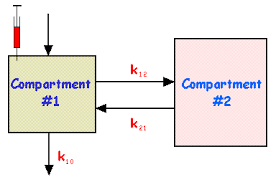
\includegraphics{2c.png}
\caption{two-compartment system}
\end{figure}

\begin{figure}
\centering
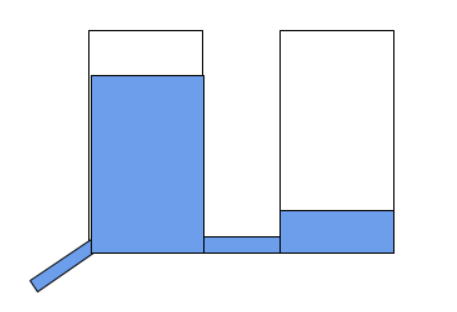
\includegraphics{2v.png}
\caption{hydraulic analogue}
\end{figure}

\begin{figure}
\centering
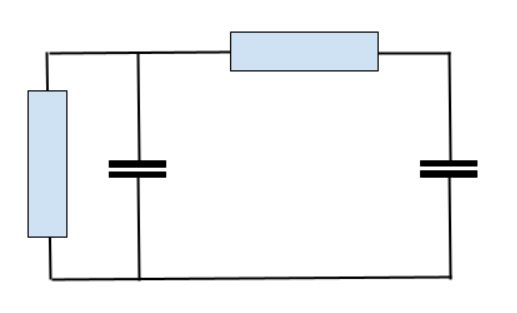
\includegraphics{2RC.png}
\caption{electrical analog}
\end{figure}

Note that the differential equations for these 3 systems are identical.
Also, the differential equations can be solved analytically using
standard methods.
\end{frame}

\begin{frame}{Significance of a compartment with a fixed rate of
removal}
\protect\hypertarget{significance-of-a-compartment-with-a-fixed-rate-of-removal}{}
In a standard S(E)IR model, disease progression is defined as:

\[\frac{\partial I}{\partial t} = \frac{-I}{d}\]

with d the duration of the infectious period (i.e.~a removal rate of
\(\frac 1 d\))

This means that although the average duration of disease equals \(d\),
\(63 \%\) \(\left (\frac 1 e \right)\) of the people in disease stage
\(I\) would have moved out in a time period shorter than \(d\). The
residence time is exponentially distributed (cf a Poisson process with a
fixed probability of an event per unit time). This is very different
from e.g.~a normal distribution. Also, infectious diseases are usually
modeled as Markov processes, which means that the change in state only
depends on the current state (i.e.~there is no memory).
\end{frame}

\end{document}
